\documentclass{article}
\usepackage{amsmath}
\usepackage{amsthm}
\usepackage{amsfonts}
\usepackage{amssymb}
\usepackage{bbold}
\usepackage{dsfont}
\usepackage{graphicx}
\usepackage{cleveref}
\usepackage{bm}
\usepackage{booktabs}
\usepackage{siunitx}
\usepackage{xcolor}
\usepackage{pdfpages}
\usepackage[utf8]{inputenc}
\usepackage[english]{babel}
\newtheorem{definition}{Definition}
\newtheorem{example}{Example}
\newcommand{\exP}[1]{\mathrm{e}^{#1}}
\newcommand{\dif}{\mathrm{d}}
\renewcommand{\vec}[1]{\mathbf{#1}}
\newcommand{\pdagger}{{\phantom{\dagger}}}
\newcommand{\state}[1]{\vert #1\rangle}
\newcommand{\cstate}[1]{\langle #1\vert}
\newcommand{\tr}[1]{\mathrm{tr}\left\{#1\right\}}
\newcommand{\trs}[2]{\, \mathrm{tr}_{#1}\{#2\}}
\newcommand{\expc}[3]{\langle #1\vert #2 \vert #3\rangle}
\usepackage[doi=false,url=false,isbn=false,backend=bibtex,style=nature,natbib=true,sorting=none]{biblatex}
\bibliography{bib.bib}
\usepackage{geometry}
\geometry{
	a4paper,
	total={170mm,257mm},
	left=15mm,
	right=15mm,
	top=15mm,
}
\begin{document}
\title{Nachtrag zum Meeting}
\author{Rudolf Smorka}
\maketitle
\section*{To do}
\begin{itemize}
	\item[1.] SOC potential: Vary $a$ and $c$. Which parameters does Fransson use? What are realistic values?
	\item[2.] For $\omega=\SI{50}{\milli\electronvolt}$ and $t_1=\SI{20}{\milli\electronvolt}$ (report 8), compare pure electronic with TTHEOM with MFHEOM. If influence of vibrations is significant: Use TAMEN code of Raffaele. Is there any improvement?
	\item[3.] Increase statistics for the MFHEOM cases from previous report. Propagate longer to steady state for $V=85$. 
	\item[4.] Fix energy conservation issue in spin-PLDM code
\end{itemize}
\section{Spin-orbit coupling potential}
Parameters as in the MFHEOM computations from previous report. As can be seen in the figure, the ratio of the helix radius $a$ to the helix pitch $c$ is relevant only, not their absolute values. Fransson uses $a/c=1$. For $a/c \approx 0.1$, the maximum of the spin-orbit coupling is approximately $\SI{0.4}{\milli\electronvolt}$, whereas for $a/c$ it is $\SI{0.125}{\milli\electronvolt}$.
\begin{figure}[!h]
	\centering
	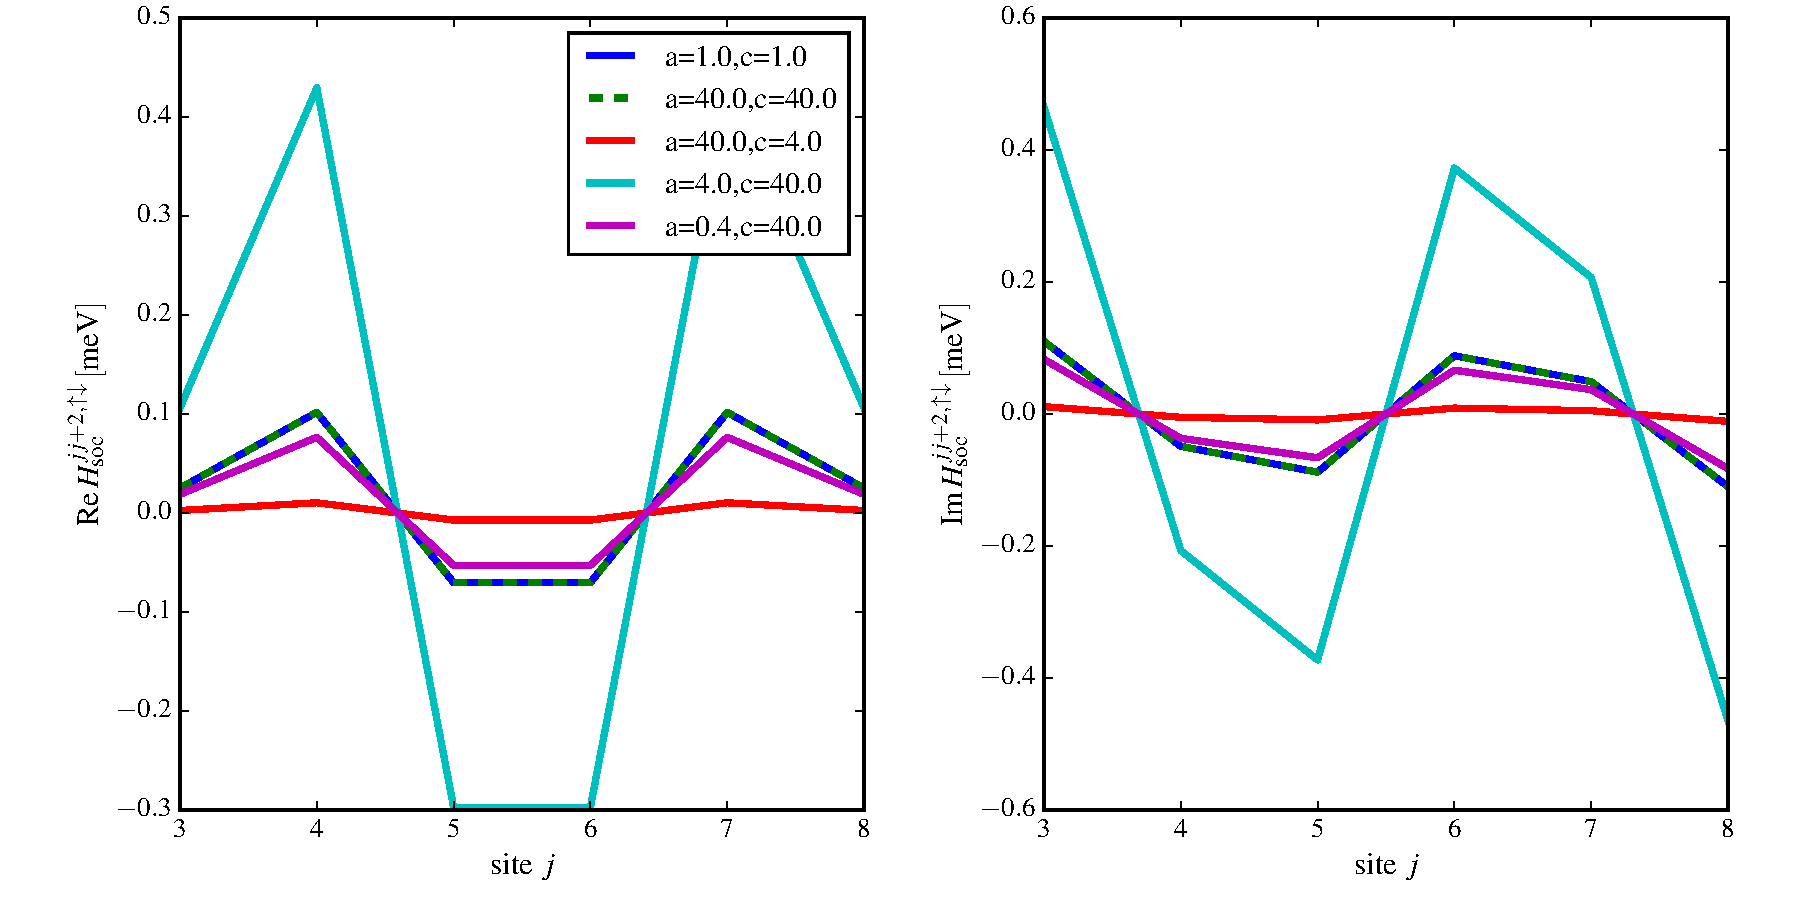
\includegraphics[width=1.0\textwidth]{figs/SOC_pot/SOC_2x4_aVar_cVar.pdf}
	\caption{Variation of $a$ (helix radius) and $c$ (helix pitch): Real (left) and imaginary (right) part of spin-orbit coupling Hamiltonian.}
\end{figure}\\
\begin{figure}[!h]
	\centering
	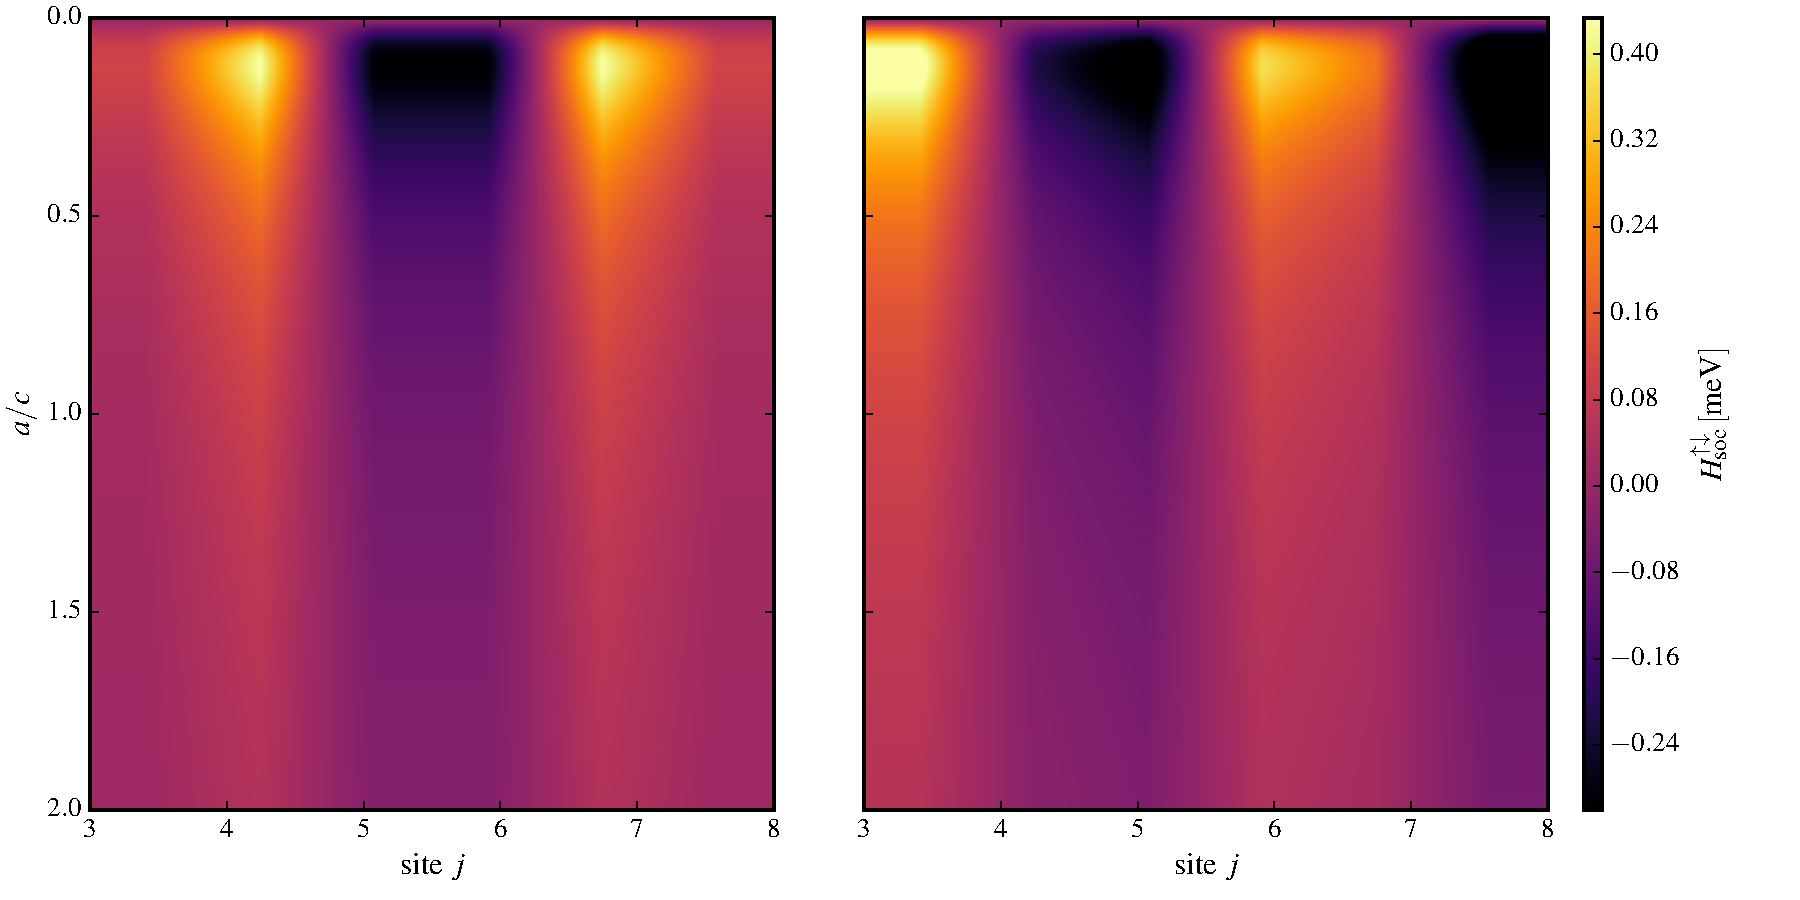
\includegraphics[width=1.0\textwidth]{figs/SOC_pot/SOC_2x4_aVar.pdf}
	\caption{Variation of $a$: Real (left) and imaginary (right) part of spin-orbit coupling Hamiltonian for $L=2\times 4$.}
\end{figure}
\begin{figure}[!h]
	\centering
	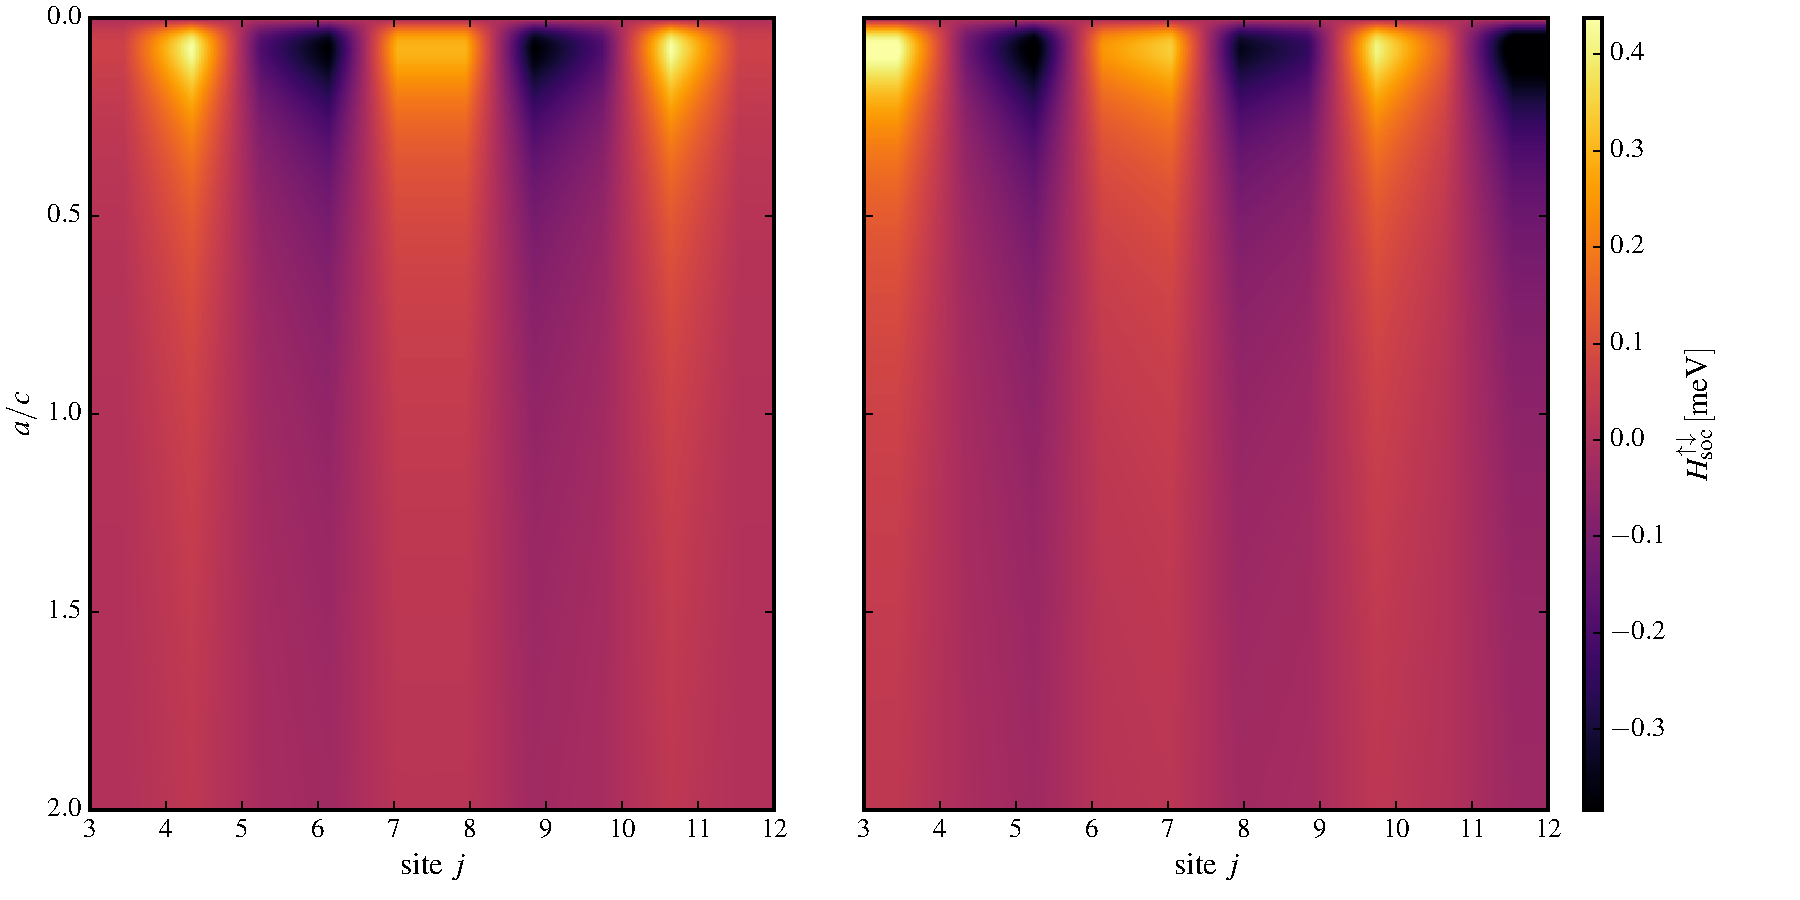
\includegraphics[width=1.0\textwidth]{figs/SOC_pot/SOC_3x4_aVar.pdf}
	\caption{Variation of $a$: Real (left) and imaginary (right) part of spin-orbit coupling Hamiltonian for $L=3\times 4$.}
\end{figure}
\end{document}


